\documentclass[12pt, twoside, a4paper]{scrbook}


\usepackage[utf8]{inputenc}
\usepackage[numbers, round]{natbib}
\usepackage{ngerman, eurosym, tikz, listings, scrhack, pdfpages, lscape, graphicx, hyperref, color}

\hypersetup{colorlinks=true, linkcolor=black, urlcolor=blue}

\usetikzlibrary{shapes, arrows}
\tikzstyle{startstop} = [rectangle, rounded corners, minimum width = 3cm, text centered, draw = black, fill = red!30]
\tikzstyle{io} = [trapezium, trapezium left angle = 70, trapezium right angle = 110, minimum width = 3cm, minimum height = 1cm, text centered, draw = black, fill = blue!30]
\tikzstyle{process} = [rectangle, minimum width = 3cm, minimum height = 1cm, text centered, draw = black, fill = orange!30]
\tikzstyle{decision} = [diamond, minimum width = 3cm, minimum height = 1cm, text centered, draw = black, fill = green!30]
\tikzstyle{arrow} = [thick, ->, >=stealth]


\author{Caspar Friedrich\\Geboren am 16. Oktober 1986\\Mat.-Nr. 11062078}
\date{Köln, den \today}
\publishers{Betreut durch Prof. Dr. Klaus Ruelberg\\Zweitprüfer: Prof. Dr. Luigi LoIacono}
\subtitle{Bachelorarbeit im Fachbereich Medienproduktionstechnik an der Fachhochschule Köln}
\title{Webgestütztes GPIO Management am Beispiel des BeagleBone Black}


\begin{document}
\maketitle
\tableofcontents
\listoffigures
\listoftables

\chapter{Einleitung}
Das \textit{Internet of Things} ist ein rasant wachsender Anwendungsbereich. Angetrieben durch eine zunehmende Akzeptanz digitaler Systeme und durch eine günstige Entwicklung in Baugröße, Leistung und Zuverlässigkeit und nicht zuletzt im Preis haben dazu geführt, dass   digitale Systeme heute in allen Lebensbereichen anzutreffen sind.
Durch die Annäherung der Hardware-Hersteller an die \glqq Hobby\grqq -Entwickler und dem Erfolg von Arduino und Co. ist der Entwicklungsaufwand eigener Hardware-Projekte erheblich kleiner als noch vor wenigen Jahren.


\section{Zielsetzung}
Nach dieser Entwicklung ist es naheliegend, auch den Laboralltag zu digitalisieren und die Verschiedenen Anforderungen und Aufgaben auf einem einzigen flexibelen System zu realisieren.

Ziel dieser Arbeit ist es dabei ein Steuersystem für Messanwendungen zu schaffen, das sich einfach konfigurieren lässt, flexibel in der Anwendung ist und gleichzeitig kostengünstig bleibt. Besonderes Augenmerk soll dabei auf der ausreichenden Verfügbarkeit verschiedener GPIO\footnote{General Purpose Input/Output} liegen. Insbesondere Pulsbreitenmodulation und Analog/Digital-Konverter sind für Messanwendungen interessant. Die anfallenden Messdaten sollen protokolliert werden und extern verwendbar sein. Die zu entwickelnde Applikation soll auf keinen bestimmten Anwendungsfall hin spezialisiert sein sondern dem Endanwender die Möglichkeit geben sich eine für sein Projekt passende Umgebung zusammen zu stellen. Weiter soll das System auch autark, vor allem über das Internet, arbeiten können. Es soll möglich sein eine entfernte Messtation auf zu bauen, die nach belieben via LAN, WLAN oder auch GSM konfiguriert und überwacht werden kann.\\

[GRAFIK!!!]


\section{Definitionen}
In dieser Arbeit wird ein \textbf{BeagleBone Black Rev. A5C} verwendet. Andere Versionen des Boards sind, sofern kompatibel, ebenfalls verwendbar allerdings nicht getestet. Um eine gut Lesabrkeit zu ermöglichen ist mit \glqq BeagleBone\grqq ~im Folgenden immer diese Version gemeint. 


\part[Grundlagen]{Grundlagen der verwendeten Technologien und Hardware}

\chapter{Hardware}

\section{Single-board Computer (SBC)}
Ein Single Board Computer oder auch SBC, zu deutsch ein Einplatinenrechner, ist ein Computersystem bei dem alle für die Verwendung nötigen Bauteile auf einer einzelnen Platine verbaut sind. Hierbei sind sind neben den essenziellen Komponenten wie Prozessor, RAM und ROM auch Controller für verschiedene I/O-Schnittstellen, Oszillatoren oder Co-Prozessoren verbaut. Single Board Computer werden vor allem in der Industrie als Steuersysteme eingesetzt, da sie oft billiger und flexibler sind als fest verdrahtete Steuersysteme. Mit zunehmender Miniaturisierung und steigender Leistungsfähigkeit finden SBC's heute auch in alltäglichen Geräten wie Autos, Waschmaschienen oder Fernbedienungen verwendung.\\

Technisch gesehen sind auch erste Heimcomputer wie der \emph{C64} oder \emph{Atari ST} Single Board Computer, allerdings lassen sich diese ohne Ein- und Ausgeabegräte wie Maus, Tastatur, Bildschirm nicht sinnvoll einsetzen und werden in der Regel nicht als solche Bezeichnet.

\subsubsection{Schnittstellen}
Single Board Computer verfügen, je nach Anwendungsgebiet, über eine Vielzahl verschiedener analoger und digitaler I/O-Schnittstellen.\\

Übliche Schnittstellen sind

\begin{itemize}
  \item Digitale IOs
  \item PWM
  \item Analog/Digital Converter (ADC)
  \item UART\footnote{Hierüber ist eine Implementierung der verbreiteten RS232/422/485-Schnittstelle möglich und auch üblich}
  \item SPI
  \item I$^{2}$C
\end{itemize}

Aktuelle (Entwickler-)Systeme haben in der Regel einen oder mehrere USB-Anschlüsse (sowohl Client als auch Host Ports sind üblich), oder zumindest einen JTAG-Port, was die Programmierung wesendlich vereinfacht. Des weiteren verfügen leistungsstärkere Systeme oft auch über einen Grafikausgang\footnote{Meist HDMI oder eine der Miniaturvarianten}.\nocite{weiser1991}

\section{System on a Chip (SOC)}
Eng verknüpft mit der Entwicklung der SBC ist das Konzept der System-on-a-Chip bzw. SOC. Hierbei werden die meisten oben genannten Komponenten eines Systems direkt in einem Einzelnen IC verbaut. Meist sind nur ROM und Controller für höhere Schnittstellen USB oder LAN (in manchen Fällen auch Grafik) extern angebunden.\\

Heutige Single-board Computer mit einem SOC können sehr leistungsstark sein, sind als Mehrkernsystem aufgebaut und haben Taktraten von mehreren GHz. Diese Computer sind vom Design her stark an Desktop-Systeme angepasst und können oft mit einem vollwertigen Linux- oder Windows-System betrieben werden.

Gerade bei diesen leistungsstarken SOCs hat sich die ARM-Architektur durchgesetzt. 1983 als Nebenprojekt gegründet hatte die 32-Bit-Architektur bereits 2002 einen Marktanteil von fast 80\% \cite{stiller2002}\\

Single Board Computer lassen sich (sehr) grob in zwei Klassen unterteilen:

\begin{enumerate}
\item \textbf{Leistungsschwache Systeme}\\
Die Taktraten dieser Prozessoren liegen überlicherweise unter 50MHz, in seltenen Fällen über 100MHz. Diese Systeme werden meist direkt programmiert und finden vor allem im low energy-Sektor anwendung.
\item \textbf{Leistungsstarke Systeme}\\
Hier ligen die Taktraten meist im GHz-Bereich. Hauptanwendungsbereiche sind Mobilfunksysteme und embedded computing in der Industrie. Gerade im Mobilfunkbereich sind oft Mehrkernsysteme anzutreffen und es wird bis auf wenige Ausnahmen oberhalb eines Betriebssystems, meist Linux bzw. Android, programmiert.
\end{enumerate}


\subsection{BeagleBone Black}
Für diese Arbeit verwende ich einen BeagleBone Black Rev. A5C (im Folgenden BeagleBone), Ein quelloffenes Entwickler-Board Mit einem ARM\textregistered ~Cortex\texttrademark -A8 Prozessor (Single Core) von Texas Instruments.\\

Die wichtigsten Features:
\begin{itemize}
  \item 1GHz Taktrate
  \item 512MB DDR3 RAM
  \item 2GB\footnote{4GB ab Rev. C} Onboard Flash Memory
  \item 10/100 Mbit/s Ethernet
  \item 69\footnote{Laut Dokumentation. 27 sind ohne weitere Konfiguration direkt verfügbar} GPIO mit mehreren PWM-Ausgängen und analogen Eingängen.
  \item Verhältnismäßig geringer Preis von ca. \EUR{45}
\end{itemize}


\chapter{Betriebsysteme}
Da die Recourcen des BeagleBone Black sehr begrenzt sind, wird für diese Arbeit ein schlankes Betriebssystem benötigt, welches nur wenig Speicher benötigt und geringen Leistungs-Overhead verursacht. Für diesen Zweck gibt es spezielle Versionen der bekannten Betriebssysteme wie Microsoft Windows oder Linux sowie verschiedene \glqq uinxoide\grqq Betriebssysteme.

\section{Linux}
Linux hat den Vorteil, dass nahzu alle Software als source code verfügbar ist und im Zweifel angepasst werden kann. Zu dem ist es üblich Lizenzen zu verwenden, die eine nicht-komerzielle Anwendung sowie Anpassungen kostenfrei zulassen.

Ein eigenes Linux zu entwickeln oder ein \textit{build system}\footnote{Einige Distributionen verwenden ein sog. build system bei dem die benötigten Kernel-Module und Software-Pakete selbst zusammengestellt werden können.} zu verwenden wäre aus Sicht der Performance sicherlich die beste Wahl und ist auch in der Industrie weitgehend üblich, würde allerdings den Rahmen dieser Arbeit sprengen. Zu dem gibt es einige sehr schlanke und bereits für den BeagleBone angepasste Linux Distributionen.

\subsection{Linux Distributionen}
BeagleBoard.org bietet auf für den BeagleBone Black zwei verschiedene Distributionen an: {\AA}ngström und Debian. Beide Distributionen haben ihre Vor- und Nachteile. Ein weiteres Projekt, welches sich unter Entwicklern großer Beliebtheit erfreut ist Arch Linux, welches auch als Basis für diese Anwendung dienen soll.

\paragraph{The {\AA}ngström Distribution} ist auf dem BeagleBone vorinstalliert und stellt die Hauptdistribution dar. Diese Distribution nutzt ein build system und findet im wesendlichen Anwendung bei Speichersystemen wie NAS oder FTP-Server, wichtigstes feature ist daher der geringe Leistungs- und Speicherbedarf. Bei dieser Distribution muss allerdings nahezu jede nicht-standard Software selbst kompiliert und eigerichtet werden.

\paragraph{Debian Linux} gilt im allgemeinen ans (rock-)stable und ist eine der verbreitetsten Distributionen, zu dem basieren einige weitere namhafte Distributionen aud Debian Linux. Stärke und gleichzeitig auch Schwäche dieser Distribution sind die langen und umfangreichen Softwaretests. Wenn ein Paket in den offiziellen repositories verfügbar ist kann man zwar davon ausgehen, dass es fehlerfrei funktioniert und zu allen anderen angebotenen Pakete kompatibel ist, allerdings liegt es meist nicht mehr in der aktuellen Version vor. Das kann gerade bei Software aus dem Bereich Netzwerk/Internet problematisch werden.

\paragraph{ArchLinux} Arch Linux hat gegenüber den oben genannten Distributionen zwei wesendliche Vorteile: Zum einen gibt es eine (Sub-)Distribution speziell für ARM-Prozessoren, bei der das Basissystem mit ca. 500MB sehr schlank ist und zum anderen ein sehr umfangreiches software repository mit sehr hoher Aktulaität. Zusätzlich gibt es das \textit{Arch User Repository}, ein freies Repository in dem jeder Nutzer seine Pakete einstellen kann. Sämtliche in diesem Projekt verwendete Software lässt sich entweder direkt aud den offiziellen Repositories installieren oder aus den User Repositories kompilieren. Zwar kann es durchaus passieren, dass die eingestellte software nicht out-of-the-box funktioniert aber in der sehr aktiven Community hinter Arch Linux bekommt man relativ schnell Hilfe.

Arch Linux ARM verwendet ein sog. \textit{Rolling Release}\footnote{Kontinuierliche Software-Entwicklung bei der Pakete separat aktuell gehalten und weiter entwickelt werden, gibt keine explizite Betriebssystemversion (Wikipedia)} es ist daher wesendlich einfacher das System aktuell und sicher zu halten. Da die Kernel-Entwicklung derzeit sehr schnell vorran schreitet, wird praktischerweise, zusätlich zur regulären Kernel-Entwicklung,   ein legacy-Paket mit einer stabilen Version gepflegt. Es muss nach einem Update des Kernel-Paketes nicht erst die Kompatibilität wieder hergestellt werden.


\chapter{Webtechnologien}

\section{Webserver}
Was ist ein Webserver? Welche sind die verbreitetsten und was sind ihre Besonderheiten.
\subsection{Lighttpd}
Warum wird Lighttpd verwendet?

\subsection{Weitere Webserver}
\paragraph{Apache}

\section{WebSockets}

\subsection{WebSockets vs. PHP}

\section{Node.js}
Was ist Node.js, wie wird es verwendet.


\part{Konfiguration des Betriebssystems}

\chapter{Betriebssystem}
Abweichend von der regulären Kernel-Entwicklung wird ein etwas älterer Kernel der Version 3.8 verwendet. Dieser wird über das Paket \textit{legacybla} bereitgestellt.

\chapter{Zusätzliche Software}
Zusätzlich zu den mitgelieferten Pakteten der Distribution werden noch ein HTTP server, ein FTP server und die JavaScript/Node.js engine benötigt. Zusätzlich wird noch ein Proxy server benötigt um mit geringem Aufwand SSL-Verschlüsselte Verbindungen zu ermöglichen und nach außen über einen einzigen Netzwerk-Port zu kommunizieren zu können.

\paragraph{haproxy} HAProxy ist ein Proxy server, der eigentlich eingesetzt wird um TCP-Anfragen auf mehrere Server zu verteilen. Wesendlich interessanter für diese Arbeit ist allerdings, dass der HAProxy nativ SSL-Verschlüsselte Verbindungen verarbeiten kann und dabei in der Basis sehr leicht zu konfigurieren ist.\cite{kuehnast2014}

In diesem wird wird HAProxy eingesetzt um WebSocket requests von regulären HTTP requests zu trennen und auf unterschiedliche Dienste weiterzuleiten. Ziel dieser Maßnahme ist es nach außen die gesamte Website hinter einem Port zu betreiben obwohl die beiden Prozessen völlig von einander getrennt sind. So ist die gefahr, dass, bei einem Feldeinsatz, der Port für den WebSocket server von einer Firewall blockiert wird minimal. Die website ist entweder vollständig oder überhaupt nicht zu erreichen. Auch ist der der WebSocket server, der systembedingt mit root-Rechten laufen muss, ausschließlich per WebSocket über den Proxy zu erreichen und ist so gegenüber Angriffen von außen weitgehend sicher.

Ein weiterer wichtiger Punkt ist, dass sich für jeden Server die maximale Anzahl der aktiven Verbindungen bequem per Config File einstellen lassen. So kann ohne besondere Programmierung sichergestellt werden, dass immer nur eine Verbindung zum WebSocket server besteht. Alle weiteren verbindungsanfragen werden auf eine Warteliste gesetzt und weitergeleitet sobald der Websocket Server wieder frei wird.

\paragraph{lighttpd} Lighttpd ist ein sehr leichtgewichtiger Webserver, der 

\paragraph{vsftpd} Ein ftp-server...

\section{nodejs}
Zusätzlich zu den von Google mitgelieferten Modulen werden noch einige Module benötigt um einen WebSocket Server zur verfügung zu stellen und die Steuerung der GPIO zu übernehmen.

\paragraph{ws} Eine der einfachsten aber auch eine der schnellsten (wenn nicht die schnellste) WebSocket-Implemtierung. WS wird von vielen komplexeren WebSocket-Modulen als Grundlage bzw. als WebSocket-Unterstützung verwendet. Das Modul ist sehr einfach zu verwenden, fehlende Funktionalität gegenüber z. B. \emph{Socket.IO} fällt in diesem Projekt nicht ins Gewicht, da der Webserver separat via Lighttpd zur Verfügung gestellt wird.

\paragraph{shelljs}

\subsubsection{bonescript}
Beschreibung der bonescript\footnote{https://github.com/jadonk/bonescript} library.


\part{Implementierung}

\chapter{Implementierung}
Das webinterface besteht im aus zwei Teilen: Einem WebSocket server, der die Steuerung der GPIO erledigt und einem Webserver, der die Dokumente ausliefert.

\section{boneserver}
Der WebSocket server ist via Node.js implementiert und und verwendet die \textit{bonescript\footnote{https://github.com/jadonk/bonescript}} library zur steuerung der GPIO.

\section{Webinterface}

\begin{figure}
  \centering
  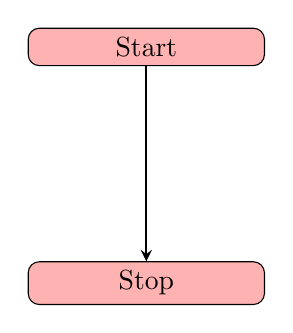
\begin{tikzpicture}[node distance = 3cm]
  \node (start) [startstop] {Start};
  \node (stop)  [startstop, below of=start] {Stop};

  \draw [arrow] (start) -- (stop);
  \end{tikzpicture}
  \caption{Test figure}
\end{figure}

\part[Fazit]{Fazit und Erweiterungsmöglichkeiten}

\appendix
\part{Anhang}

\chapter{Tabellen}

\begin{landscape}
  \begin{table}
  \centering
  \includegraphics[page=1, trim=14mm 19mm 14mm 19mm, clip=true, scale=0.8]{doc/BeagleboneBlackP8HeaderTable.pdf}\\
  \tiny by Derek Molly (www.derekmolloy.ie)
  \caption{BeagleBone Black Expansion Header (P8)}
  \end{table}
\end{landscape}

\begin{landscape}
  \begin{table}
  \centering
  \includegraphics[page=1, trim=8mm 26mm 8mm 25mm, clip=true, scale=0.8]{doc/BeagleboneBlackP9HeaderTable.pdf}\\
  \tiny by Derek Molly (www.derekmolloy.ie)
  \caption{BeagleBone Black Expansion Header (P9)}
  \end{table}
\end{landscape}

\bibliographystyle{plaindin}
\bibliography{literatur}


\end{document}
